\documentclass[../../spr.tex]{subfiles}

\begin{document}


\section{Implementacja}

\subsection{Opis głównych funkcjonalności aplikacji}

\begin{itemize}
  \item autoryzacja z wykorzystaniem OIDC.
  \item Płatności.
  \item zarządzanie siłownnią
\end{itemize}

\subsection{Prezentacja zrzutów ekranu (screeny) prezentujących działanie aplikacji}
\begin{figure}[H]
  \centering
  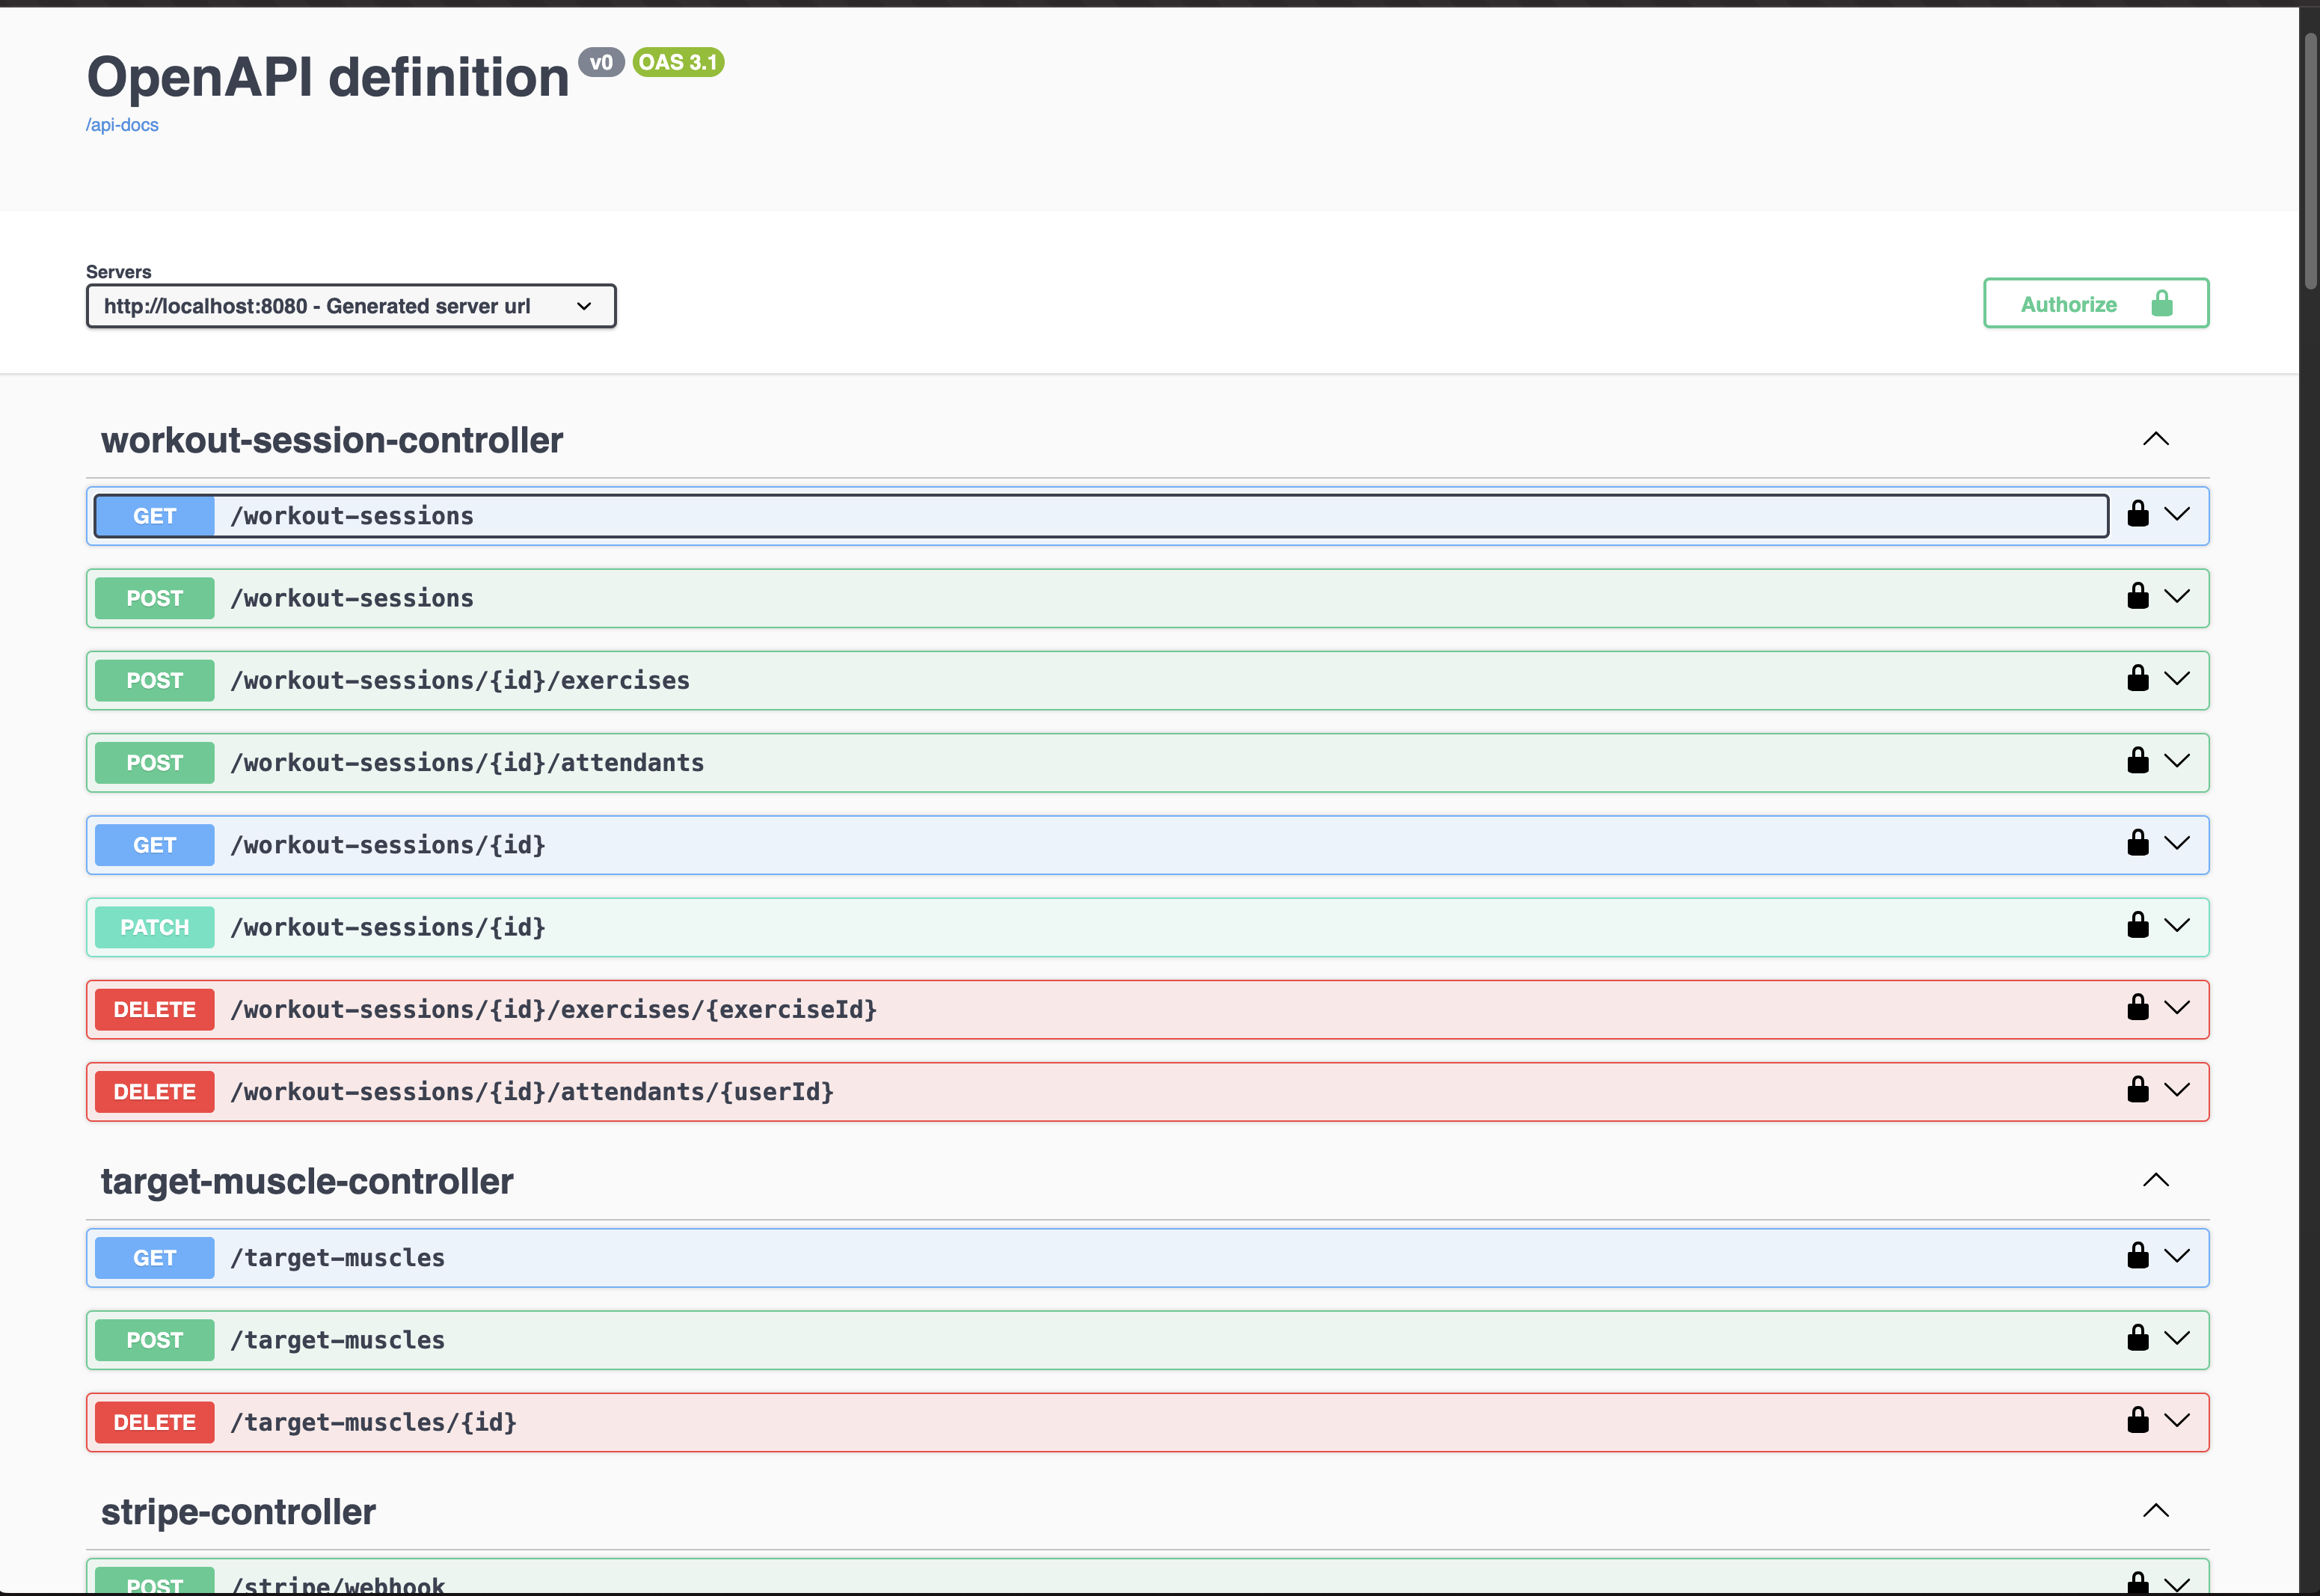
\includegraphics[width=\textwidth]{swagger.png}
  \caption{Swagger UI z dokumentacją API}
\end{figure}

\subsection{Wybrane fragmenty kodu z kluczowymi funkcjonalnościami}


\subsubsection{Autoryzacja z tokena JWT}

\captionsetup{hypcap=false}
\begin{center}
  \inputminted[
    breaklines,
    fontsize=\footnotesize,
    breakanywhere,
    numbers=left
  ]{java}{./sections/implementacja/GymJwtAuthenticationConverter.java}
  \captionof{listing}{Autoryzacja z tokena JWT (OIDC)}
\end{center}


\begin{center}
  \inputminted[
    breaklines,
    fontsize=\footnotesize,
    breakanywhere,
    numbers=left
  ]{java}{./sections/implementacja/HallController.java}
  \captionof{listing}{Przykładowy kontroler}
\end{center}

\begin{center}
  \inputminted[
    breaklines,
    fontsize=\footnotesize,
    breakanywhere,
    numbers=left
  ]{java}{./sections/implementacja/HallServiceImpl.java}
  \captionof{listing}{Przykładowy serwis}
\end{center}

\begin{center}
  \inputminted[
    breaklines,
    fontsize=\footnotesize,
    breakanywhere,
    numbers=left
  ]{java}{./sections/implementacja/HallControllerTest.java}
  \captionof{listing}{Przykładowe testy jednego z kontrolerów}
\end{center}

\subsubsection{}

\end{document}